%!TEX root = ../../main.tex


\begin{figure}[!htb]
\centering
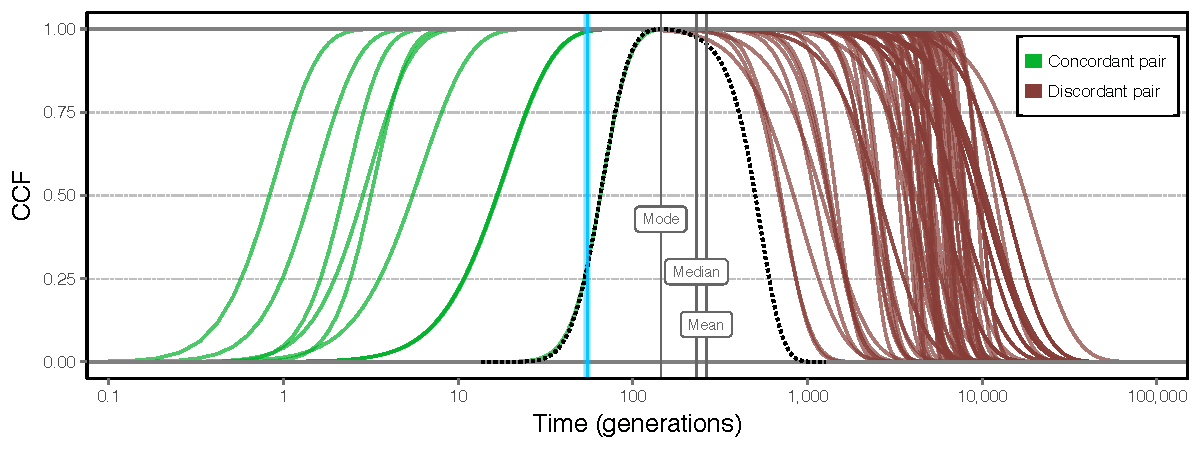
\includegraphics[width=\textwidth]{./img/ch5/age_example}
\Caption{Example of the age estimation result for a focal variant}%
{A target variant was randomly selected from simulated data.
Each of the possible concordant pairs was formed and analysed using the \gls{ccf}.
A subset of ${n_d = \num{100}}$ discordant pairs was randomly selected and analysed using the \gls{ccf}.
Vertical lines indicate the mode, median, and mean of the composite likelihood distribution.
The \emph{blue} line marks the true age of the mutation, as determined from simulation records.}%
{fig:age_example}
\end{figure}
